% Supplementary material for "Position-Faithful Merge Tree Maps: Certified Bounds and Near-Optimal Layouts".
% Compile: `tectonic -X compile supplement.tex` (or pdfLaTeX + BibTeX). Figures and tables from scripts/make_figures.py.
\documentclass[10pt]{article}
\usepackage[margin=2cm]{geometry}
\usepackage[T1]{fontenc}
\usepackage{mathptmx}
\usepackage{graphicx,booktabs,amsmath,amssymb,amsthm}
\usepackage[hidelinks]{hyperref}
\newtheorem{lemma}{Lemma}
\newtheorem{theorem}{Theorem}
\newtheorem{proposition}{Proposition}
\newcommand{\dtop}{d_{\mathrm{top}}}
\newcommand{\lca}{\operatorname{lca}}
\newcommand{\nroe}{\mathrm{NROE}}
\renewcommand{\thesection}{S\arabic{section}}
\renewcommand{\thefigure}{S\arabic{figure}}
\renewcommand{\thetable}{S\arabic{table}}
\title{Supplementary Material\\[2pt]\large Position-Faithful Merge Tree Maps: Certified Bounds and Near-Optimal Layouts}
\author{Anonymous Authors}
\date{}
\begin{document}\sloppy
\maketitle

Theorem numbers refer to the paper. Notation: $T_t$ is the merge tree of step $t$ (join convention; apply everything to $-f$ for superlevel sets), $V_{ij}=f(\lca(i,j))$, $q_i\in[0,L]$ the reference of leaf $i$, $W_i$ its interval width, $g$ the gap, $H_i=\rho W_i/2$ the anchor slack, $\dtop$ the labelled merge error (Eq.~2 of the paper) and $\Delta_F$ the scalar range. All claims below were also checked against exhaustive enumeration on random trees (\texttt{code/tests/test\_order\_certificate.py}, \texttt{code/tests/test\_interval\_order.py}).

\section{Proofs}

\paragraph{Interval model.} For a leaf order $\pi$, leaf $k$ occupies $[c_k-W_k/2,\,c_k+W_k/2]\subseteq[0,L]$; consecutive intervals do not overlap and are at least $g$ apart; the anchor satisfies $|x_k-c_k|\le H_k$. If leaf $a$ precedes leaf $b$ and every leaf of a set $S\ni a,b$ lies between them (inclusive), then
\begin{equation}\label{eq:pack}
c_b-c_a\ \ge\ \sum_{k\in S}s_k-g-\tfrac{W_a}{2}-\tfrac{W_b}{2},\qquad s_k=W_k+g,
\end{equation}
because the half intervals of $a$ and $b$, the full intervals of the leaves between them and one gap per consecutive pair fit between the two centres; leaves of the order that are not in $S$ only add distance. The attained cost is $\tau(\pi)=\min\max_k|x_k-q_k|$ over all such placements.

\begin{theorem}[Theorem 2 of the paper]
Let $\ell_k=q_k-W_k/2-H_k$, $h_k=q_k+W_k/2+H_k$, and for a leaf set $S$ let $A(S)=\max_\alpha[\alpha+\sum_{k\in S,\ell_k\ge\alpha}s_k]$ and $B(S)=\max_\beta[\sum_{k\in S,h_k\le\beta}s_k-\beta]$, the maxima taken over $\alpha\in\{\ell_k\}$, $\beta\in\{h_k\}$. (i) If every leaf of $X$ precedes every leaf of $Y$, then $\tau\ge(A(X)+B(Y)-g)/2$. (ii) Every placement satisfies $\tau\ge B(\mathrm{all})-g$ and $\tau\ge A(\mathrm{all})-g-L$. (iii) With $W\equiv0$ and $g=0$, the bound of (i) over sibling pairs equals $L\,\nu^*$.
\end{theorem}
\begin{proof}
(i) Take $S_X\subseteq X$, $S_Y\subseteq Y$, let $a$ be the first leaf of $S_X$ and $b$ the last leaf of $S_Y$ in the order. All of $S=S_X\cup S_Y$ lies between them, so by (\ref{eq:pack}) and the anchor slack, $x_b-x_a\ge\sum_S s_k-g-W_a/2-W_b/2-H_a-H_b$. Since $\tau\ge q_a-x_a$ and $\tau\ge x_b-q_b$,
\[
\tau\ \ge\ \tfrac12\big[(q_a-x_a)+(x_b-q_b)\big]\ \ge\ \tfrac12\Big[\ell_a-h_b+\sum_{k\in S}s_k-g\Big]\ \ge\ \tfrac12\Big[\min_{S_X}\ell+\sum_{S_X}s_k+\sum_{S_Y}s_k-\max_{S_Y}h-g\Big].
\]
For $S_X=\{k\in X:\ell_k\ge\alpha\}$ the first two terms are at least $\alpha+\sum_{k\in X,\ell_k\ge\alpha}s_k$; for $S_Y=\{k\in Y:h_k\le\beta\}$ the last ones are at least $\sum_{k\in Y,h_k\le\beta}s_k-\beta$. The two choices are independent, so maximizing each gives $A(X)$ and $B(Y)$. Each maximum is over upper (resp.\ lower) sets of one sorted list and is computed by one sort and a prefix sum.
(ii) Let $b$ be the last leaf of a set $S$. The intervals of $S$ lie in $[0,c_b+W_b/2]$, so $c_b\ge\sum_S s_k-g-W_b/2$, $x_b\ge c_b-H_b$ and $\tau\ge x_b-q_b\ge\sum_S s_k-g-h_b\ge\sum_S s_k-g-\max_S h$. Lower sets of $h$ give $B(\mathrm{all})-g$. The right end is symmetric with the first leaf of $S$ and gives $A(\mathrm{all})-g-L$.
(iii) Then $\ell=h=q$, $s=0$, $A(X)=M_X$, $B(Y)=-m_Y$, and $\min(A(X)+B(Y),A(Y)+B(X))/2=\min(M_X-m_Y,M_Y-m_X)/2$, which is $L$ times the term of $\nu^*$.
\end{proof}

\begin{lemma}[Separated sets]\label{lem:sets}
If no element of $Q$ lies strictly between two elements of $P$ in a linear order, and no element of $P$ lies strictly between two elements of $Q$, then all of $P$ precedes all of $Q$ or vice versa.
\end{lemma}
\begin{proof}
All of $Q$ lies outside the span of $P$. If $Q$ had elements on both sides of that span, all of $P$ would lie strictly between two elements of $Q$.
\end{proof}

\begin{theorem}[Theorem 3 of the paper]
Let $A_\varepsilon(u)$ be the highest ancestor of $u$ with $f(A_\varepsilon(u))\le f(u)+2\varepsilon$. In every map with $\dtop\le\varepsilon$: (i) no leaf outside $A_\varepsilon(u)$ lies between two leaves of $u$; (ii) if no leaf of $w$ is in $A_\varepsilon(u)$ and no leaf of $u$ is in $A_\varepsilon(w)$, then all leaves of $u$ precede all leaves of $w$ or vice versa. Consequently $\nroe\ge\frac1{2L}\max\min(M_u-q_k,\,q_k-m_u)$ over leaves $k\notin A_\varepsilon(u)$, $\nroe\ge\frac1{2L}\max\min(M_u-m_w,\,M_w-m_u)$ over pairs as in (ii), and the same pairs give width-aware bounds on $\tau$ through Theorem~2(i), with $A(\{k\})=\ell_k+s_k$ and $B(\{k\})=s_k-h_k$ for a single leaf.
\end{theorem}
\begin{proof}
(i) For a leaf $k$ outside $A_\varepsilon(u)$ and any leaf $i$ of $u$, $\lca(i,k)$ is a proper ancestor of $A_\varepsilon(u)$, so $V_{ik}>f(u)+2\varepsilon$ by the choice of $A_\varepsilon(u)$; by Lemma~1 of the paper, $k$ cannot lie between two leaves of $u$. (ii) By (i) applied to $u$ and to $w$, the conditions of Lemma~\ref{lem:sets} hold for their leaf sets. The bounds follow as in the proofs of Theorems~1 and~2(i), since those only used that one set precedes the other.
\end{proof}

\paragraph{The coarse bound.} If a node $u$ has parent level above $f(u)+2\varepsilon$, then $A_\varepsilon(u)=u$ and $u$ is contiguous by Theorem~3(i). Hence in every map with $\dtop\le\varepsilon$ the children of each node of $T^{(2\varepsilon)}$ (all nodes within $2\varepsilon$ of their parent flattened) occupy disjoint blocks, and Theorems~1 and~2 apply to $T^{(2\varepsilon)}$. The chain bound contains every pair used here and is never weaker.

\paragraph{Data resolution.} Treating levels closer than $\varepsilon_0\Delta_F$ as equal is the statement $\dtop\le\varepsilon_0\Delta_F$ for the ties; all bounds hold with $\varepsilon_0+\varepsilon$ in place of $\varepsilon$.

\begin{proposition}[Optimal barriers]
Fix an order $\pi$ and the extremum values. For the gap $k$ between the $k$th and $(k{+}1)$st leaf let $C_k=\min\{V_{\pi(i)\pi(j)}: i\le k<j\}$ and $F_k=\max(f(\pi(k)),f(\pi(k{+}1)))$. The smallest achievable merge error is
\[
\delta^*(\pi)=\max\Big(0,\ \max_{i<j}\tfrac12\big(V_{\pi(i)\pi(j)}-\max_{i\le k<j}C_k\big),\ \max_k(F_k-C_k)\Big),
\]
attained by the barriers $b_k=C_k+\delta^*(\pi)$.
\end{proposition}
\begin{proof}
The displayed merge of the $i$th and $j$th leaf is $\max_{i\le k<j}b_k$, and each barrier must be at least $F_k$ to keep both basins. An error $\delta$ requires $b_k\le V_{\pi(i)\pi(j)}+\delta$ for every pair spanning $k$, i.e., $b_k\le C_k+\delta$; it also requires $\max_{i\le k<j}b_k\ge V_{\pi(i)\pi(j)}-\delta$ and $b_k\ge F_k$. The largest admissible barriers $b_k=C_k+\delta$ satisfy all constraints exactly when $\delta$ is at least each term of $\delta^*$; smaller barriers only lower the maxima. Hence $\delta^*$ is optimal and attained.
\end{proof}

\section{Methods and protocol}
\paragraph{Ordering details.} Candidate trees: the exact tree; one tree per distinct parent gap $s\le2(\varepsilon_0+\varepsilon)$ with every node within $s$ of its parent flattened; and a conflict-driven flattening that repeatedly releases one or both nodes of the sibling pair with the largest order cost if the chain condition of Theorem~3 holds and the exact $\delta^*$ of the resulting midpoint order stays within the budget. The four best candidates by initial $\tau$, plus the exact tree, are refined by local search: for every node, all insertions of one child block at another position (all of them up to eight children, otherwise within distance three), accepted when they lower $(\tau,\sum\text{positive terms}^2)$ and keep $\delta^*\le(\varepsilon_0+\varepsilon)\Delta_F$; at most eight passes. On 300 random trees with widths, this search reached the exhaustive optimum of $\tau$ on 296; the point-model order on 250.

\paragraph{Metrics.} SNS, TW ($k=1$), TD and ME follow the protocol of the completed nine-input table of our earlier evaluation and of ST-MTM: unweighted support centroids in the native spatial dimension; positions on the full $[0,1]$ canvas; motion events over two steps whose source distance changes by more than 2\% of the domain diagonal, judged with a display threshold of 2\% of the occupied range (fixed canvas for Cylinder). Planar domain diagonals are not stored; we use the midpoint of the interval that reproduces the stored event count, and thresholds are nested, so the whole interval selects the same events. Recomputing the stored baselines from their saved anchors agrees exactly in SNS and TD except Cylinder (relative $10^{-5}$), in TW to the third or fourth decimal on Tangaroa and Cylinder, and in ME up to one event on PM$_{2.5}$, Ring and Cylinder; the stored values were taken from rendered anchors.

\paragraph{Instances.} Given the native branch decisions, the TMTM linearization matched the pinned official C++ core in all 3127 arc intervals and anchors of the five planar sequences (687, 431, 289, 463, 1257), with zero merge error. Native ST-MTM anchors and intervals satisfied the KKT conditions of ST-MTM Eqs.~1--2 with relative residuals at most $3.6\cdot10^{-8}$ and $9.6\cdot10^{-7}$ (planar) and stationarity residuals at most $7.1\cdot10^{-11}$ (volumetric). SciPy optimal leaf ordering exceeded the exhaustive optimum of its adjacency objective on 1, 7, 0, 2 and 0 frames of Storms, Wildfires, OLR, PM$_{2.5}$ and Ring. Enumerating all $2^k$ branch decisions against the same previous greedy layout, TMTM's greedy step was optimal at 36/39, 47/59 and 351/365 steps of Ring, OLR and PM$_{2.5}$; summed over steps it exceeded the per-step optimum by 17.4\%, 5.7\% and 2.2\%.

\paragraph{Labelled interleaving.} We checked the conditions of the identification $\dtop=d_I^L$ against arXiv:1908.00063: labels must cover all leaves (labels on inner vertices are allowed), the induced matrix includes the diagonal $f(\pi(i))$, and $d_I^L$ is defined as the $\ell_\infty$ distance of induced matrices. Every column of the rendered Ring and OLR maps has exactly one local extremum per feature (0 exceptions in 200 columns), so no unlabelled leaf occurs there.

\paragraph{Runtime.} Apple M2 Pro (12 cores, 32\,GB), macOS 26.6, Python 3.12.7, NumPy 2.0.2, SciPy 1.13.1, one process. Per frame: bounds 0.11--0.62\,ms (planar) and 2.7--5.5\,ms (volumetric); ordering 0.40--3.7\,ms and 11--103\,ms; capped QP 2.3--9.0\,ms and 0.25--0.50\,s.

\section{Additional results}

\begin{table}[h]
\caption{All values of the cross-method comparison (paper Fig.~6), in percent except SNS and TW.}\label{tab:compare}
\centering\small
\begin{tabular}{llrrrrr}\toprule
Sequence & Method & NROE & worst merge & ME & SNS & TW\\\midrule
\csname @@input\endcsname tables/tab_compare.tex 
\bottomrule\end{tabular}
\end{table}

\begin{table}[h]
\caption{Order error and position (percent). $\nu^*$ and mean NROE of native TMTM, ST-MTM and our exact layout; mean and worst displacement of our capped layouts; worst displacement and worst merge error (NMLE max) at $\varepsilon=2\%$ and $10\%$.}\label{tab:main}
\centering\small\setlength{\tabcolsep}{4pt}
\begin{tabular}{lrcrrrrrr|rr|rr}\toprule
 & & & \multicolumn{4}{c}{NROE} & \multicolumn{2}{c|}{$\varepsilon=0$} & \multicolumn{2}{c|}{$\varepsilon=2\%$} & \multicolumn{2}{c}{$\varepsilon=10\%$}\\
Sequence & Frames & Leaves & $\nu^*$ & TMTM & ST-MTM & Ours & $E_{\mathrm{pool}}$ & $E_\infty$ & $E_\infty$ & NMLE & $E_\infty$ & NMLE\\\midrule
\csname @@input\endcsname tables/tab_main.tex 
\bottomrule\end{tabular}
\end{table}

\begin{table}[h]
\caption{Volumetric sequences (percent). $\kappa$ P (exact) and R2 (relaxed, no merge-error cap): earlier construction. N1: certified order by NROE only. Jump: mean $|\Delta x-\Delta q|/L$ of matched features.}\label{tab:volume}
\centering\small
\begin{tabular}{llrrrrr}\toprule
 & Layout & $E_{\mathrm{pool}}$ & $E_\infty$ & NROE & jump & NMLE max\\\midrule
\csname @@input\endcsname tables/tab_volume.tex 
\bottomrule\end{tabular}
\end{table}

\begin{table}[h]
\caption{Reference direction in 3-D (percent): mean order bound $\nu^*$, mean NROE of our exact width-aware order, ST-MTM and TMTM (native orientation chosen in their favour), and mean attained displacement $\tau/L$ of our order with its width-aware lower bound, for the coordinate axes, the stored direction and the direction with the smallest bound among 400.}\label{tab:direction}
\centering\small\setlength{\tabcolsep}{4pt}
\begin{tabular}{llrrrrrr}\toprule
Sequence & Direction & $\nu^*$ & Ours & ST-MTM & TMTM & $\tau/L$ & bound\\\midrule
\csname @@input\endcsname tables/tab_direction.tex
\bottomrule\end{tabular}
\end{table}

\begin{figure}[h]
\centering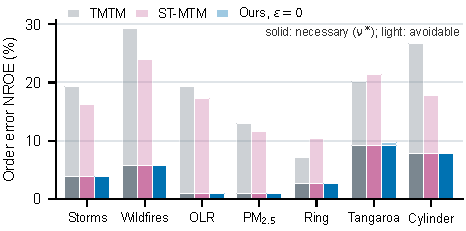
\includegraphics[width=.6\linewidth]{figures/fig_bound.pdf}
\caption{Mean order error per sequence split into the necessary part $\nu^*$ (solid) and the avoidable remainder (light).}
\end{figure}

\begin{figure}[h]
\centering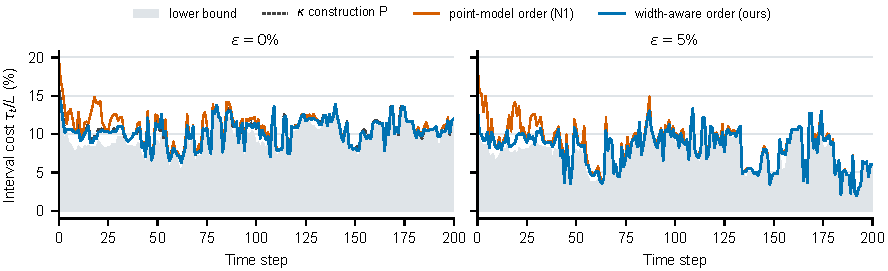
\includegraphics[width=\linewidth]{figures/fig_tangaroa.pdf}
\caption{Tangaroa, 201 steps: interval cost $\tau_t/L$ of the point-model order (orange), the width-aware order (blue) and the $\kappa$ construction (dashed), with the certified lower bound (grey).}
\end{figure}

\begin{figure}[h]
\centering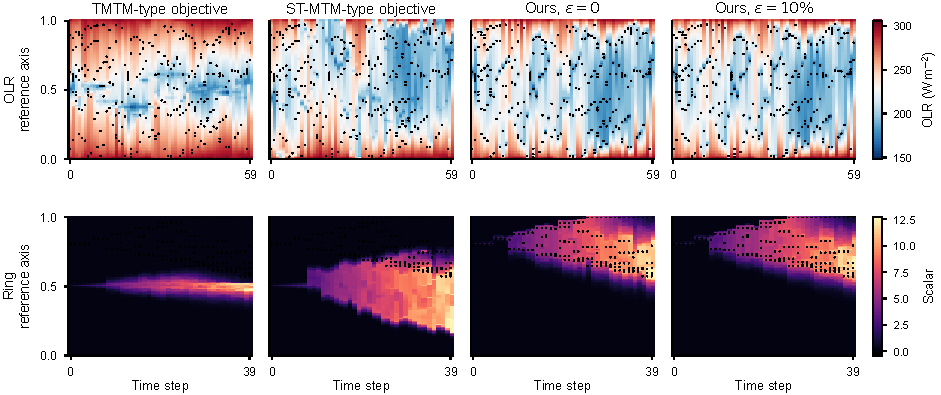
\includegraphics[width=\linewidth]{figures/fig_maps.pdf}
\caption{OLR (60 days) and Ring (40 steps) maps that differ only in the layout objective; dots mark references.}
\end{figure}

\end{document}
